\documentclass[12pt, a4paper, oneside]{mwart} % Z automatu 10pt w przypisach
\usepackage[utf8]{inputenc} % Znaki diakrytyczne z klawiatury
\usepackage[OT4]{fontenc} % OT4 ponizej nie dzialalo
\usepackage[plmath,MeX]{polski} % Ponoc lepsza polonizacja LaTeXa
%\usepackage[dvips]{graphicx}
\usepackage[pdftex]{color,graphicx} % Grafika w PDFowej formie
%\usepackage{dcolumn} % Wyrownywanie przecinka w tabelach
%\newcolumntype{d}[1]{D{.}{,}{#1}} % Typ kolumny do wyrownywania
%\usepackage{threeparttable} % Coby ladnie podpisac tabelki
%\usepackage{rotating} % for sidewaystable
%\usepackage{subfig}

\usepackage[pdftex]{hyperref} % Zarzadza hiperlaczami w dokumencie, ostatni w preambule, dvips/pdftex zaleznie od wyjscia

\begin{document}
\title{
\includegraphics[width = 0.3 \textwidth]{wykresy/SGHlogotypCMYKpl.eps}\\
\bigskip
Zaawansowane Modelowanie Symulacyjne [234060-0723]\\ 
\bigskip
PiTU~S.A.\\
Symulacja portfela ubezpieczeń komunikacyjnych}
\author{Anna Chojnacka, 68729 (budowa modelu) \and
Michał Puchalski, 67827 (analiza wrażliwości) \and
Paweł Sadłowski, 68404 (edycja raportu)}
\date{Warszawa, 1.04.2018}
\maketitle

\begin{abstract}
Przedmiotem raportu jest ryzyko niewypłacalności związane z~portfelem ubezpieczeń komunikacyjnych. Przy wyjściowym poziomie składki równym 500~PLN oszacowane prawdopodobieństwo bankructwa wynosi~0.627, zdecydowanie przekraczając akceptowalny poziom. Na~podstawie wyników symulacji rekomendujemy ustalenie składki w~wysokości 1500~PLN, która przy nadwyżce początkowej równej 10~000~PLN zapewnia prawdopodobieństwo niewypłacalności nieprzekraczające 1\%. Wnioski pozostają w~znacznej mierze niezmienione nawet w~przypadku wahania przeciętnej liczby zgłaszanych szkód o~$\pm$5\%. Wyniki są~również stabilne z~uwagi na~liczbę iteracji modelu.
\end{abstract}

\pagebreak

\section{Opis~organizacji}
PiTU S.A. to~zakład ubezpieczeń specjalizujący~się w~ubezpieczeniach komunikacyjnych. Jego~aktywność jest skoncentrowana w~Bryczkolandii. Firma należy do~liderów silnie skoncentrowanego rynku, jej ubiegłoroczne przychody wyniosły niespełna 243~tys.~PLN. Najsilniejszą presję konkurencyjną wywiera lokalny zakład ubezpieczeń z~dużym udziałem własnościowym skarbu państwa oraz trzy mniejsze filie korporacji zagranicznych.

\section{Opis problemu}
Kraj, w~którym PiTU~S.A. prowadzi swoją działalność, notuje rosnącą imigrację z~sąsiedniego Dżydżykistanu. Z~uwagi na~naturalnie wyższą skłonność do~zachowań ryzykownych u~przedstawicieli tej~narodowości firma spodziewa~się wzrostu szkodowości, w~związku z~czym przewiduje konieczność podniesienia składki. Celem przeprowadzonej symulacji jest wyznaczenie odpowiedniej wysokości składki zabezpieczającej towarzystwo ubezpieczeniowe przed niewypłacalnością. Zakres analizy obejmuje także ocenę wrażliwości nadwyżki końcowej oraz prawdopodobieństwa niewypłacalności na~wysokość nadwyżki początkowej oraz pobieranej składki.

\subsection{Szczegółowy scenariusz symulacji}

\begin{table}
\centering
\caption{Rozkład szkód zgłaszanych przez Dżydżyków}
\label{r_szkod}
\begin{tabular}{p{1cm}|l||r|l}
\multicolumn{2}{c||}{Liczba~szkód}&\multicolumn{2}{c}{Wysokość szkody}\\ \hline
0&3 437&100&0\\
1&522&200&2\\
2&40&500&27\\
3&2&1 000&52\\
4&0&2 000&115\\
5&0&5 000&203\\
&&10 000&106\\
&&20 000&42\\
&&40 000&14\\
&&50 000&0\\
&&55 000&0\\
&&60 000&1\\
\end{tabular}
\end{table}

\begin{figure}
\centering
\caption{Rozkład liczby szkód oraz wysokości szkody}
\label{rozklad_szkod}
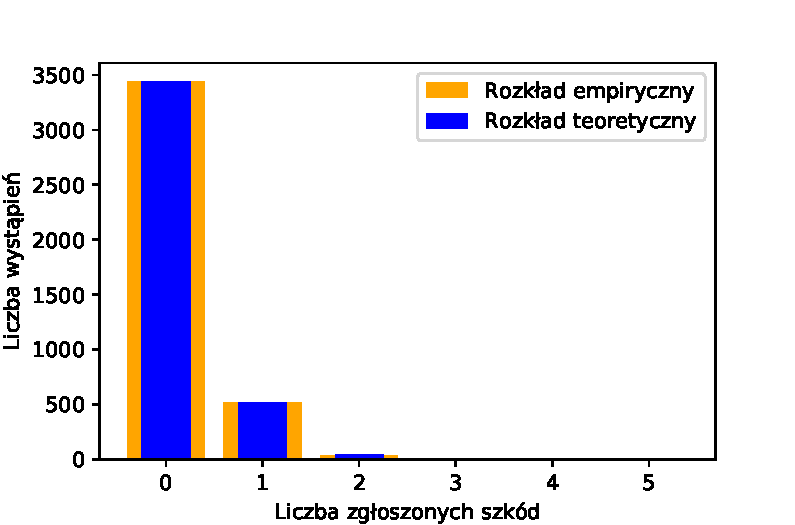
\includegraphics[width = \textwidth]{wykresy/rozklad_l_szkod.pdf}
\newline
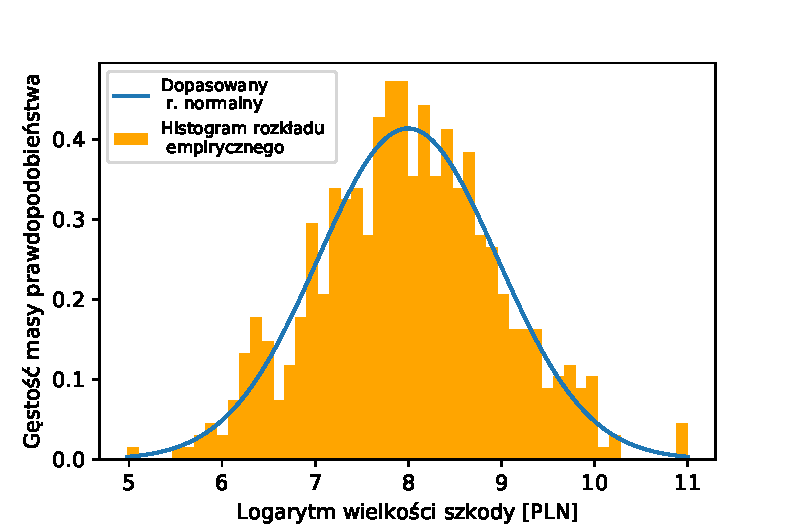
\includegraphics[width = \textwidth]{wykresy/rozklad_wys_szkody.pdf}
\end{figure}

Firma PiTU~S.A. dysponuje historycznymi danymi dotyczącymi liczby oraz wielkości szkód zgłaszanych przez klientów dżydżyckiej narodowości~(\cite{case}). Przekazane informacje zostały ujęte w tabeli~\ref{r_szkod}. Prezes zarządu spodziewa~się portfela liczącego ok.~100 polis, a~bieżąca nadwyżka wynosi 10~000~PLN. Dział~Aktuarialny PiTU~S.A. rekomenduje przybliżanie liczby szkód przez rozkład Poissona, a~ich wysokości przez rozkład log-normalny. Przedstawione dane nie~dają podstaw do~odrzucenia tych założeń --- do~ich weryfikacji zastosowano odpowiednio: test $\chi^2$ oraz test Kołmogorowa-Smirnowa. W~obu przypadkach p-value znacznie przekraczało 0.9, więc zgodnie z~literaturą przedmiotu~(\cite{mielczarek}) wykorzystanie w~procesie modelowania wymienionych rozkładów można uznać za~uzasadnione. Horyzont czasowy analizy został ustalony na~dwa lata.

\subsection{Struktura modelu}
Zgodnie z~terminologią zastosowaną przez Averilla Lawa (\cite{law}) zastosowany model jest przykładem symulacji zdarzeń dyskretnych (discrete-event simulation). Modelowanym zjawiskiem jest wielkość nadwyżki w~dyspozycji zakładu ubezpieczeniowego w~poszczególnych dniach. W~każdej iteracji symulacji ustalona liczba klientów (100) wykupuje polisę ubezpieczeniową w~trakcie pierwszego roku. Dla każdego z~klientów data zawarcia umowy jest losowana z~rozkładu jednostajnego (dyskretnego). Następnie dla każdego klienta losowane są: liczba szkód (z~rozkładu Poissona), a~także data wystąpienia (ponownie z~dyskretnego rozkładu jednostajnego) oraz wysokość każdej z~nich (rozkład log-normalny) --- o~ile wystąpią. Wszystkie wymienione zmienne losowane są~niezależnie od~pozostałych. Ostatecznie stan nadwyżki jest obliczany na~każdy kolejny dzień w~horyzoncie czasowym symulacji, z~uwzględnieniem wpływów ze~składek oraz wydatków na~pokrycie szkód. W~przypadku gdy dowolnego dnia suma szkód przekracza wartość dostępnej nadwyżki, dochodzi do~niewypłacalności. W~przeciwnym razie model zwraca stan nadwyżki na~koniec okresu symulacji. 

\section{Wyniki analizy}
Przedstawione w~dalszej części wyniki oraz wnioski są oparte na~rezultatach symulacji, w~której każdy zestaw parametrów był podstawą 1000 iteracji modelu. W~następnym kroku rezultaty zostały zagregowane dla~poszczególnych wartości parametrów.

\subsection{Wysokość składki a prawdopodobieństwo bankructwa}
Wyniki analizy jednoznacznie wskazują, że~składka w~wysokości 500~PLN nie~pokrywa ryzyka wystąpienia szkód w~wystarczającym stopniu --- prawdopodobieństwo niewypłacalności wyniosło 0.627.

\begin{figure}
\centering
\caption{Prawdopodobieństwo bankructwa dla poszczególnych wysokości składki}
\label{p_bankructwa_n1000}
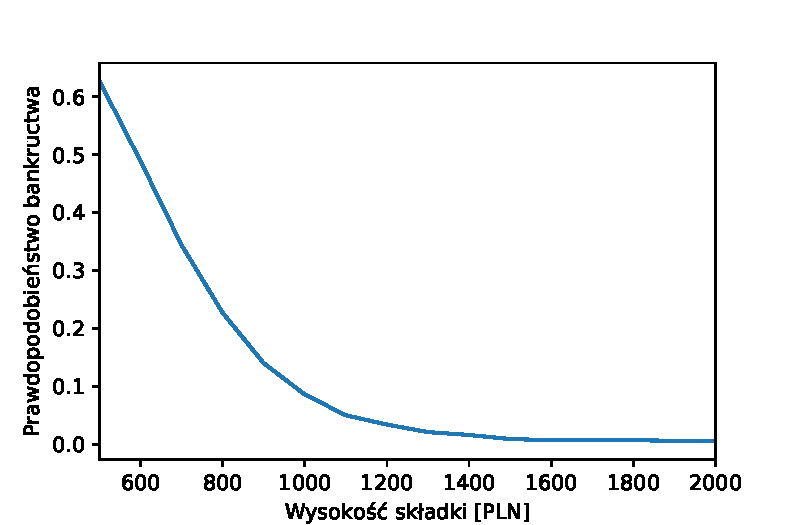
\includegraphics[width = \textwidth]{wykresy/p_bankructwa.pdf}
\end{figure}

\begin{figure}
\centering
\caption{Prawdopodobieństwo bankructwa nieprzekraczające 1\%}
\label{p_heatmapa_bankructwo_mniej_niz_0,01}
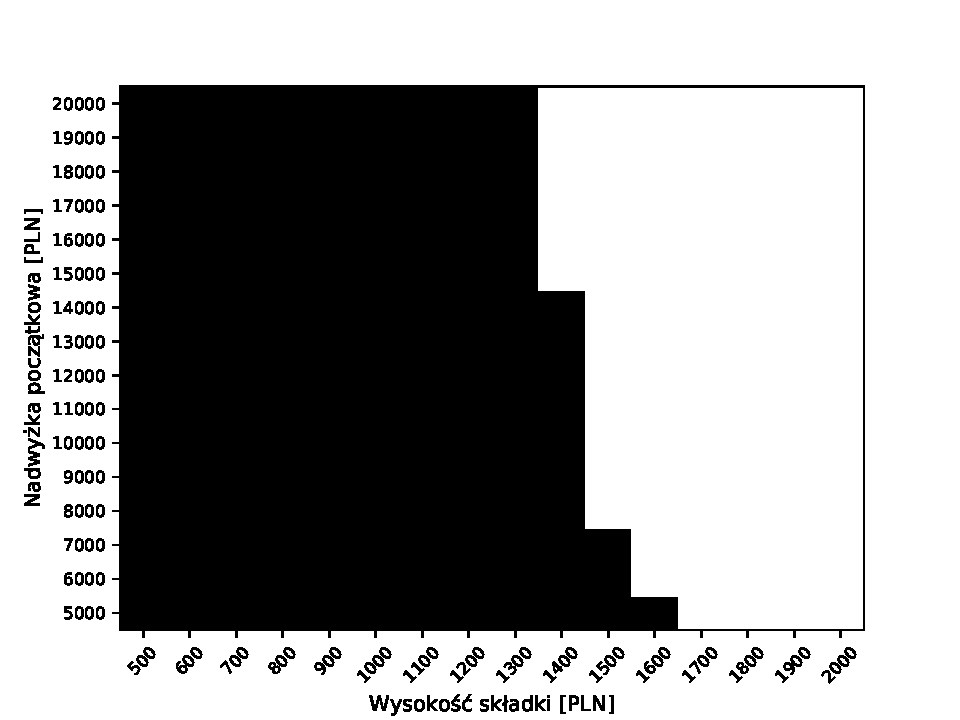
\includegraphics[width = \textwidth]{wykresy/p_heatmapa_bankructwo_mniej_niz_0,01.pdf}
\footnotesize Białymi polami oznaczono kombinacje parametrów, dla~których prawdopodobieństwo niewypłacalności nie~przekroczyło 0.01.
\end{figure}

Wykres~\ref{p_bankructwa_n1000} ilustruje zależność pomiędzy wysokością składki a~prawdopodobieństwem bankructwa. Krzywa ma~kształt hiperboliczny, co~oznacza, że~podnoszenie składki poprawia perspektywy zakładu ubezpieczeniowego w~coraz mniejszym stopniu. Wybór~optymalnej wysokości składki powinien zatem równoważyć niskie prawdopodobieństwo bankructwa oraz niski poziom składki, tak~aby zniechęceni klienci nie~zdecydowali~się na~konkurencyjną ofertę. Punkt załamania krzywej znajduje~się w~okolicach składki wynoszącej 1000~PLN. Prawdopodobieństwo niewypłacalności wynosi wówczas niespełna 10\%, a~co za~tym idzie --- wciąż jest duże. Najmniejszą wysokością składki, dla~której nie~przekracza ono poziomu 1\% jest 1500~PLN. Wysokość składki, dla~której prawdopodobieństwo bankructwa nie~przekracza~1\%, w~zależności od~nadwyżki początkowej można prześledzić na~wykresie~\ref{p_heatmapa_bankructwo_mniej_niz_0,01}.

\subsection{Wpływ nadwyżki początkowej na prawdopodobieństwo bankructwa}
Drugim parametrem, który wpływa na~szanse utrzymania~się przez przedsiębiorstwo na~rynku jest wysokość nadwyżki początkowej. Ze~swojej natury jest~to wielkość, którą znacznie trudniej kontrolować (jej~podniesienie wymagałoby najprawdopodobniej pozyskania przez PiTU~S.A. dodatkowego finansowania), a~przy tym uzyskane efekty będą miały charakter tymczasowy --- będą w~stanie uchronić firmę przed upadłością, ale nie~przyczynią~się do~trwałego wzrostu rentowności portfela.

\begin{figure}
\centering
\caption{Porównanie prawdopodobieństw bankructwa dla~różnych poziomów nadwyżki początkowej}
\label{p_bankructwa_porownanie_n1000}
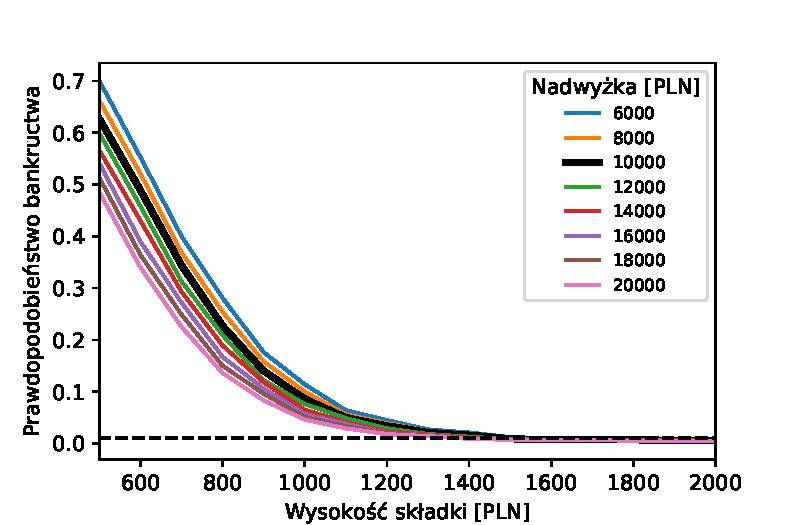
\includegraphics[width = \textwidth]{wykresy/p_bankructwa_porownanie.pdf}
\end{figure}

\begin{figure}
\centering
\caption{Prawdopodobieństwo bankructwa w~zależności od~nadwyżki początkowej i~składki}
\label{p_heatmapa_bankructwo}
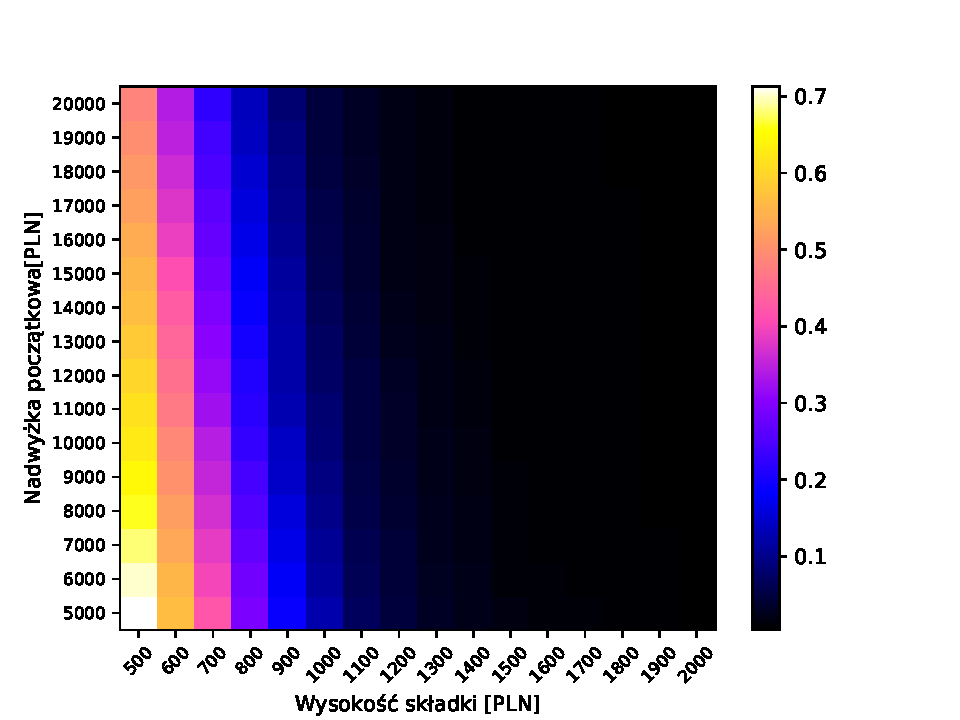
\includegraphics[width = \textwidth]{wykresy/p_heatmapa_bankructwo.pdf}
\end{figure}

Wykres~\ref{p_bankructwa_porownanie_n1000} obrazuje tę~tendencję --- wpływ nadwyżki znacząco maleje wraz ze~wzrostem rentowności portfela. Analogiczne wnioski płyną z~analizy mapy cieplnej (rysunek~\ref{p_heatmapa_bankructwo}), na~której zilustrowano prawdopodobieństwo bankructwa w~zależności od~nadwyżki początkowej oraz składki --- wyraźnie widać, że~znacznie szybciej maleje ono wraz ze~wzrostem drugiej z~tych wielkości. Z~tego powodu priorytetem powinno pozostać ustalenie składki na~poziomie gwarantującym długoterminową rentowność portfela polis ubezpieczeniowych.

\subsection{Wysokość nadwyżki końcowej}

\begin{figure}
\centering
\caption{Przeciętna nadwyżka końcowa w~scenariuszach pozytywnych dla różnych poziomów składki}
\label{nadwyzka_n1000}
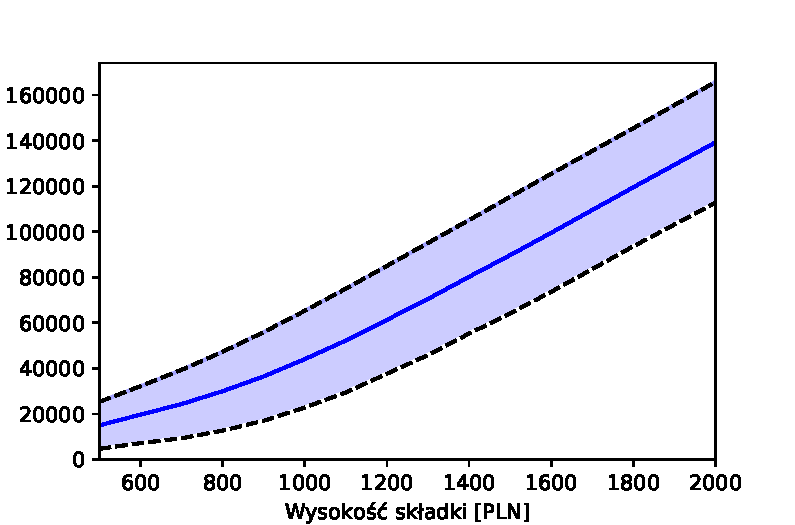
\includegraphics[width = \textwidth]{wykresy/nadwyzka.pdf}
\end{figure}

Warto zaznaczyć, że~w pozytywnych scenariuszach (tj.~gdy firma unika niewypłacalności) nadwyżka końcowa w~większości przypadków przekracza nadwyżkę początkową. Jak widać na~wykresie~\ref{nadwyzka_n1000} nawet dla składki wynoszącej 500~PLN PiTU~S.A. mogłoby oczekiwać zysku na~przeciętnym poziomie 4955~PLN, pod warunkiem że~firmie udałoby~się uniknąć niewypłacalności. Różnica pomiędzy średnią nadwyżką końcową a~nadwyżką początkową przekracza 1~odchylenie standardowe pierwszej wielkości począwszy od~składki równej 800~PLN, zaś próg dwóch odchyleń standardowych jest osiągany dla~składki równej 1200~PLN. Przy składce ustalonej na~rekomendowanym poziomie 1500~PLN~spodziewana nadwyżka końcowa wynosi 89711.37~PLN, a~jej odchylenie standardowe --- 25617.60~PLN.

\section{Analiza wrażliwości}
Wyniki symulacji zostały przeanalizowane pod~kątem wrażliwości na~dwa parametry: oczekiwaną liczbę szkód zgłaszanych przez pojedynczego klienta oraz liczbę iteracji modelu, na~podstawie której opracowane zostały wyniki.

\subsection{Błąd oszacowania szkodowości}
Naturalizacja dużej grupy obywateli Dżydżykistanu może spowodować zmianę charakterystyk populacji --- nowi klienci mogą okazać~się grupą bardziej lub~mniej ryzykowną od~dotychczasowych, przez co~oszacowanie parametru $\lambda$ w~rozkładzie Poissona nie~będzie w~adekwatny sposób odzwierciedlało ryzyka wystąpienia szkody. Należy podejrzewać, że~efekt ten będzie dotyczył raczej liczby zgłaszanych szkód niż ich~wysokości. Z~tego powodu przedmiotem analizy wrażliwości uczyniliśmy oszacowanie parametru $\lambda$, rozważając jego niedoszacowanie oraz przeszacowanie o~5\%.

\begin{figure}
\caption{Wrażliwość prawdopodobieństwa bankructwa dla~różnych wysokości składki na~zmianę średniej liczby szkód}
\label{p_bankructwa_all}
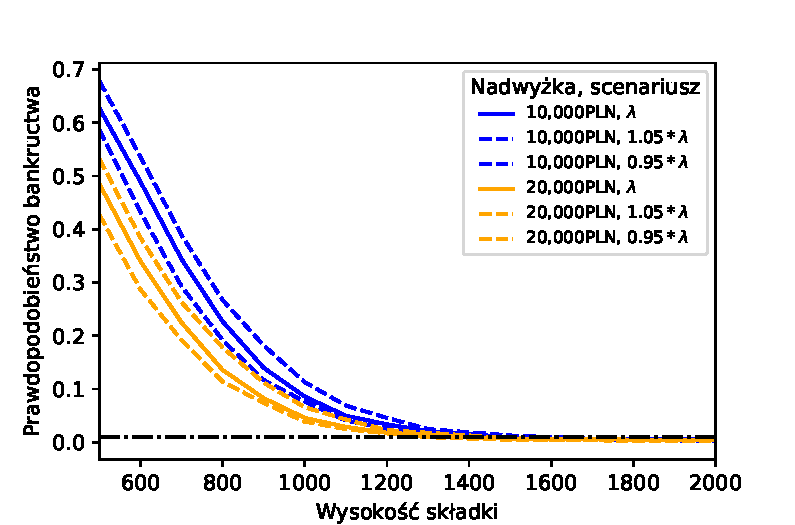
\includegraphics[width = \textwidth]{wykresy/p_bankructwa_all.pdf}
\end{figure}

\paragraph{}
Wahania parametru $\lambda$ wokół wartości oszacowanej na~podstawie dostępnych danych nie~prowadzą do~znaczących zmian rozwiązania optymalnego. W~przypadku mniejszej skłonności nowo naturalizowanych obywateli do~zachowań ryzykownych ($\lambda$ mniejsza od~pierwotnie szacowanej) 1500~PLN pozostaje poziomem, dla~którego prawdopodobieństwo bankructwa po~raz pierwszy spada poniżej~1\%. Scenariusz przeciwny powoduje, że~do~utrzymania ryzyka niewypłacalności na~poziomie nieprzekraczającym~1\% konieczne będzie ustalenie składki w~wysokości 1700~PLN. Jednocześnie jednak przy wzroście nadwyżki początkowej o~8000~PLN kwota 1500~PLN okaże~się w~zupełności wystarczająca. Szczegółową zależność pomiędzy składką a~prawdopodobieństwem niewypłacalności w~rozważanych scenariuszach można prześledzić na~wykresie~\ref{p_bankructwa_all}.

\subsection{Liczba iteracji}
Jak wspomniano wcześniej, powyższe wyniki i~rekomendacje zostały przedstawione w~oparciu o~1000~iteracji modelu dla~każdego z~rozważanych zestawów parametrów. W~ramach analizy wrażliwości przeprowadziliśmy analogiczne procedury stosując 500 iteracji za~pierwszym razem oraz 1500 iteracji w~drugim przypadku. Wnioski pozostają w~przeważającej mierze niezmienione --- w~szczególności składka w~wysokości 1500~PLN przy nadwyżce początkowej wynoszącej 10~000~PLN daje prawdopodobieństwo bankructwa nieprzekraczające~1\%. Z~uwagi na wysoką zbieżność wyników wykresy porównawcze zostały pominięte.

\section{Wnioski i zalecenia}
Na~podstawie zamieszczonych powyżej analiz rekomendujemy ustalenie składki~dla nowych klientów z~Dżydżykistanu na~poziomie 1500~PLN. W~scenariuszu bazowym zapewnia ona pokrycie potencjalnych szkód z~wysokim prawdopodobieństwem (niewypłacalność nastąpiła tylko w~0.9\% przypadków). Zgodnie z~naszymi ustaleniami to~właśnie wysokość składki stanowi kluczową zmienną decyzyjną, ze~względu na~trudności w~manipulacji oraz ograniczony wpływ nadwyżki początkowej. Wyznaczone przez nas rozwiązanie w~znacznej mierze pozostaje optymalne nawet w~przypadku zmiany charakterystyk populacji. Oferta PiTU~S.A. jest nadal konkurencyjna w~przypadku spadku szkodowości, a~jej potencjalny wzrost skutkuje prawdopodobieństwem bankructwa wyższym jedynie o~0.4~p.~proc. Dodatkowo warto zaznaczyć, że~efekt ten może zostać zniwelowany poprzez zwiększenie składki o~200~PLN bądź pozyskanie dodatkowego finansowania (wzrost nadwyżki początkowej). Rentowność portfela polis jest wysoka --- dla~rekomendowanej wysokości składki nadwyżka końcowa (wyłączając przypadki bankructwa) wynosiła przeciętnie~89711.37~PLN i~była o~ponad 3~odchylenia standardowe większa od~nadwyżki początkowej. Wnioski pozostają niezmienione w~przypadku ograniczenia liczby iteracji do~500 lub~jej~zwiększenia do~1500.

\begin{thebibliography}{9}
%\bibitem{slajdy}
%P.~Szufel, \emph{Zaawansowane Modelowanie Symulacyjne --- materiały do~wykładu}
\bibitem{law}
Averill~M.~Law, W.~David~Kelton,
\emph{Simulation Modeling \& Analysis},
McGraw-Hill, wyd.~drugie, 1991
\bibitem{case}
P.~Wojewnik, \emph{Pitu case study}
\bibitem{mielczarek}
Bożena~Mielczarek, \emph{Modelowanie symulacyjne w~zarządzaniu. Symulacja dyskretna},
Oficyna Wydawnicza Politechniki Wrocławskiej, Wrocław~2009
\end{thebibliography}

\end{document}